\documentclass{article}
\usepackage{tikz}
\usetikzlibrary{arrows.meta, positioning, shapes.geometric}
\usepackage[utf8]{inputenc}
\usepackage[UTF8]{ctex}
% \setCJKmainfont{}
\usepackage{amsmath}
\usepackage{amssymb}
\usepackage{array}
\usepackage{booktabs}
\usepackage{enumitem}
\usepackage{xeCJK}
\usepackage{CJKutf8}
\setCJKmainfont{Noto Serif CJK TC}    % 思源宋體繁體版(推薦)
\setCJKsansfont{Microsoft JhengHei}   % 微軟正黑體
\setCJKmonofont{Noto Sans Mono CJK TC}
% \setCJKmainfont{WenQuanYi Zen Hei}
% % 或者使用其他可用字體:
% % \setCJKmainfont{AR PL Mingti2L Big5}
% % \setCJKmainfont{Noto Sans CJK TC}

% % 設置全形符號支持
% \setCJKsansfont{WenQuanYi Zen Hei}
% \setCJKmonofont{WenQuanYi Zen Hei}

\title{Self-Injection-Locked (SIL) Oscillator Analysis}
\author{carlos ma}
\date{\today}

\begin{document}
\maketitle

\section{General Definition}

\textbf{Resonance} occurs when a system is subjected to an external force or signal whose frequency matches the system's \textbf{natural frequency}, resulting in a large increase in amplitude.

\section{Real-World Examples}

\begin{center}
\begin{tabular}{>{\centering\arraybackslash}m{3cm} >{\raggedright\arraybackslash}m{9cm}}
\toprule
\textbf{Context} & \textbf{Description} \\
\midrule
Violin string & Vibrates strongly when bowing matches its natural vibration frequency \\
RF circuits & LC circuits resonate at a specific frequency $\rightarrow$ used in filters, radios \\
Bridges & Tacoma Narrows Bridge collapsed due to wind-induced resonance \\
SIL radar & Resonator oscillates strongly at $\omega_n$; injection close to $\omega_n$ causes locking \\
\bottomrule
\end{tabular}
\end{center}

\section{In Engineering Terms}

For a \textbf{second-order system} like an RLC circuit or mechanical spring-mass-damper system:

\subsection{Natural Frequency}
\begin{align}
\omega_n &= \sqrt{\frac{k}{m}} \quad \text{(mechanical)} \\
\omega_n &= \frac{1}{\sqrt{LC}} \quad \text{(electrical)}
\end{align}

When driven at $\omega = \omega_n$, the system exhibits \textbf{maximum energy transfer} and large amplitude.

\section{Resonance Graphically}

If you plot amplitude vs frequency, the \textbf{resonance peak} appears at $\omega_n$, especially if the system has \textbf{high quality factor (Q)}.

\section{In Self-Injection Locked Oscillators}

In SIL systems:
\begin{itemize}
    \item The oscillator has a \textbf{resonant frequency} $\omega_n$
    \item The feedback (injection) signal, when close to $\omega_n$, causes the oscillator to \textbf{lock its frequency and phase}
    \item This locking happens more efficiently \textbf{because of resonance}
\end{itemize}

\section{Summary}

\begin{center}
\begin{tabular}{>{\centering\arraybackslash}m{4cm} >{\raggedright\arraybackslash}m{8cm}}
\toprule
\textbf{Term} & \textbf{Meaning} \\
\midrule
Resonance & Strong response when input $\approx$ natural frequency \\
Natural Frequency & The frequency a system ``prefers'' to oscillate at \\
Quality Factor (Q) & Determines how sharp/narrow the resonance is \\
\bottomrule
\end{tabular}
\end{center}

\section{Adler's Equation (Simplified Form)}
    
\begin{equation}
\frac{d\phi(t)}{dt} = \Delta \omega - K \cdot \sin(\phi(t))
\end{equation}

Where:
\begin{itemize}
    \item $\phi(t)$: phase difference between oscillator and injection signal
    \item $\Delta \omega = \omega_{\text{inj}} - \omega_0$: natural frequency difference
    \item $K$: coupling strength (determined by injection energy and oscillator Q factor)
\end{itemize}

\section{Notes for SIL Radar}

Excellent question! That equation:

\begin{equation}
\omega(t) - \omega_n \approx -\frac{\omega_n}{2Q} \cdot \frac{B}{A} \cdot \sin[\theta(t)]
\end{equation}

comes from analyzing \textbf{self-injection-locked (SIL)} oscillators --- specifically how \textbf{injection} of a reflected signal modifies the \textbf{oscillator's instantaneous frequency}.

Let me explain \textbf{step by step} how this equation is derived from the physics of a resonator-based oscillator subject to weak injection:

\subsection{Context}

\begin{itemize}
    \item $\omega_n$: natural frequency of the oscillator (free-running)
    \item $\omega(t)$: actual instantaneous frequency when injection is present
    \item $Q$: quality factor of the oscillator (higher $\rightarrow$ sharper resonance)
    \item $A$: amplitude of the oscillator signal
    \item $B$: amplitude of the injected signal (typically a reflected echo)
    \item $\theta(t)$: phase difference between injected and oscillator signals
\end{itemize}

\subsection{Step-by-step Derivation}

\subsubsection{Step 1: Start from the complex oscillator dynamics}

In oscillator theory, a sinusoidal oscillator's dynamics near resonance can be described using \textbf{complex envelope} notation:

Let the oscillator's complex amplitude be:
\begin{equation}
z(t) = A(t) e^{j\phi(t)}
\end{equation}

Assuming a self-sustained oscillator with \textbf{external injection} $B e^{j(\omega_{\text{inj}} t + \phi_B)}$, its dynamics can be modeled using a \textbf{resonator differential equation}:

\begin{equation}
\frac{dz}{dt} + \left(j\omega_n + \frac{\omega_n}{2Q}\right) z = \frac{\omega_n}{2Q} B e^{j(\omega_{\text{inj}} t + \phi_B)}
\end{equation}

Here:
\begin{itemize}
    \item The term on the left is the oscillator's natural decay and oscillation
    \item The term on the right is \textbf{external drive (injection)}
\end{itemize}

\subsubsection{Step 2: Assume steady-state, decompose phase dynamics}

Let:
\begin{itemize}
    \item $z(t) = A e^{j\omega(t)t}$
    \item Assume \textbf{injection frequency is close to $\omega_n$} $\rightarrow$ do slow-varying approximation
    \item Define $\theta(t) = \phi(t) - \omega_{\text{inj}} t$ as the phase difference between oscillator and injected signal
\end{itemize}

Then, you can extract the \textbf{phase evolution}:
\begin{equation}
\frac{d\theta}{dt} = \omega(t) - \omega_{\text{inj}} \approx \omega(t) - \omega_n
\end{equation}

That's the \textbf{phase error rate}.

\subsubsection{Step 3: Linearize injection-locking force}

From resonator theory (and RF oscillator models), the effect of injection is to ``pull'' the oscillator frequency, and that pulling is \textbf{proportional to the sine of the phase difference} $\sin(\theta)$.

From the forced oscillator dynamics and projection onto quadrature component, we get:
\begin{equation}
\omega(t) - \omega_n \approx -\frac{\omega_n}{2Q} \cdot \frac{B}{A} \cdot \sin[\theta(t)]
\end{equation}

This is the approximate \textbf{Adler-type equation} specifically for a SIL system using a resonator.

\subsection{Physical Meaning}

\begin{center}
\begin{tabular}{>{\centering\arraybackslash}m{3cm} >{\raggedright\arraybackslash}m{8cm}}
\toprule
\textbf{Term} & \textbf{Meaning} \\
\midrule
$\omega(t) - \omega_n$ & How much the oscillator's frequency is ``pulled'' \\
$\frac{\omega_n}{2Q}$ & Sets the \textbf{natural bandwidth} of the oscillator's response \\
$\frac{B}{A}$ & Strength of the injected signal relative to self-oscillation amplitude \\
$\sin(\theta(t))$ & Phase interaction term driving the frequency shift \\
\bottomrule
\end{tabular}
\end{center}

\section{Explain Adler Equation with Block Diagram}

This equation comes from:
\begin{enumerate}
    \item Resonator + injection modeling
    \item Linearized oscillator dynamics near steady-state
    \item Projection of injection onto oscillator's quadrature axis
    \item Assuming small amplitude variation (constant envelope)
\end{enumerate}

It is \textbf{more specific than Adler's equation}, applying directly to SIL oscillators with $Q$-limited resonators.

\subsection{Adler Equation Block Diagram}

% \begin{center}
    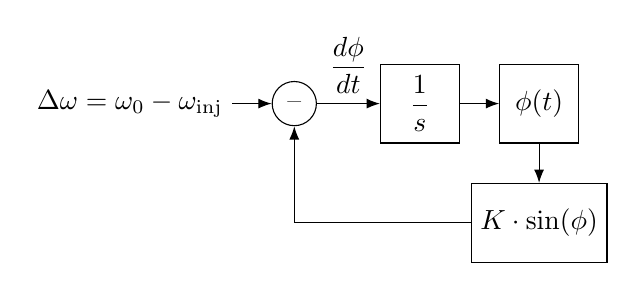
\begin{tikzpicture}[auto, node distance=2.5cm, >=Latex]

        % Nodes
        \node[left] (delta) {\( \Delta\omega = \omega_0 - \omega_{\text{inj}} \)};
        \node[draw, circle, minimum size=0/3cm, right=0.5cm of delta] (sum) {--};
        \node[draw, rectangle, minimum width=1cm, minimum height=1cm, right=0.8cm of sum] (int) {\( \dfrac{1}{s} \)};
        \node[draw, rectangle, minimum width=1cm, minimum height=1cm, right=0.5cm of int] (phi) {\( \phi(t) \)};
        \node[draw, rectangle, minimum width=1cm, minimum height=1cm, below=0.5cm of phi] (sin) {\( K \cdot \sin(\phi) \)};
      
        % Arrows
        \draw[->] (delta) -- (sum);
        \draw[->] (sum) -- node {\( \dfrac{d\phi}{dt} \)} (int);
        \draw[->] (int) -- (phi);
        \draw[->] (phi) -- (sin);
        \draw[->] (sin) -| (sum.south);
      
      \end{tikzpicture}
% \end{center}

The block diagram shows:
\begin{itemize}
    \item \textbf{Input}: Frequency difference $\Delta \omega = \omega_{\text{inj}} - \omega_0$
    \item \textbf{Nonlinear feedback}: $K\sin(\phi)$ represents injection locking force
    \item \textbf{Integrator}: Converts frequency difference to phase
    \item \textbf{Output}: Phase difference $\phi(t)$
\end{itemize}

% \usepackage{amsmath}
% \begin{left}

% \end{left}
\section*{RF信號的IQ表示法}

一個簡單的數學表示:

若原始 RF 信號為:
\[
s(t) = A(t) \cdot \cos\left(2\pi f_c t + \phi(t)\right)
\]

它可以轉換為 IQ 表示為:
\[
s(t) = I(t) \cdot \cos\left(2\pi f_c t\right) - Q(t) \cdot \sin\left(2\pi f_c t\right)
\]

其中:
\[
\begin{aligned}
I(t) &= A(t) \cdot \cos\left(\phi(t)\right) \\
Q(t) &= A(t) \cdot \sin\left(\phi(t)\right)
\end{aligned}
\]

\subsection*{舉例:16-QAM}

例如在 16-QAM(Quadrature Amplitude Modulation)中,每個符號都會有一組對應的 $I$ 和 $Q$ 值,用以決定其在星座圖(constellation diagram)中的位置。

\section{系統分類}

根據開迴路傳遞函數中積分器的個數,將系統分為:

\begin{itemize}
    \item \textbf{0型系統}:無積分器
    \item \textbf{I型系統}:有1個積分器
    \item \textbf{II型系統}:有2個積分器
\end{itemize}

\section{誤差係數與穩態誤差}

\subsection{位移誤差係數 ($K_p$)}

\begin{equation}
K_p = \lim_{s \to 0} G(s)H(s)
\end{equation}

對於單位階躍輸入 $r(t) = 1$:
\begin{itemize}
    \item 0型系統:$e_{ss} = \frac{1}{1+K_p}$
    \item I型和II型系統:$e_{ss} = 0$
\end{itemize}

\subsection{速度誤差係數 ($K_v$)}

\begin{equation}
K_v = \lim_{s \to 0} sG(s)H(s)
\end{equation}

對於單位斜坡輸入 $r(t) = t$:
\begin{itemize}
    \item 0型系統:$e_{ss} = \infty$
    \item I型系統:$e_{ss} = \frac{1}{K_v}$
    \item II型系統:$e_{ss} = 0$
\end{itemize}

\subsection{加速度誤差係數 ($K_a$)}

\begin{equation}
K_a = \lim_{s \to 0} s^2G(s)H(s)
\end{equation}

對於單位拋物線輸入 $r(t) = \frac{t^2}{2}$:
\begin{itemize}
    \item 0型和I型系統:$e_{ss} = \infty$
    \item II型系統:$e_{ss} = \frac{1}{K_a}$
\end{itemize}

\section{實際評估步驟}

\begin{enumerate}
    \item \textbf{確定系統型別}:分析開迴路傳遞函數,計算積分器個數
    \item \textbf{計算誤差係數}:根據系統型別計算相應的$K_p$、$K_v$、$K_a$
    \item \textbf{選擇測試輸入}:使用階躍、斜坡、拋物線輸入
    \item \textbf{計算穩態誤差}:利用最終值定理或誤差係數公式
    \item \textbf{時域仿真驗證}:透過數值仿真觀察實際誤差行為
\end{enumerate}

\section{改善誤差的方法}

\begin{itemize}
    \item 增加系統型別(增加積分器)
    \item 提高開迴路增益
    \item 加入前饋補償
    \item 使用PID控制器
\end{itemize}

這種系統性的分析方法能夠有效預測和改善控制系統的穩態性能。


\section{Starting Point: Simple Harmonic Oscillator}

We begin with the basic oscillator equation:

\begin{equation}
\ddot{x} + \omega_0^2 x = 0
\end{equation}

This represents a \textbf{lossless oscillator} (like a perfect spring-mass system or LC circuit).

\section{Problem: Real Oscillators Have Losses}

In reality, all oscillators lose energy due to:
\begin{itemize}
    \item \textbf{Resistance} (in electrical circuits)
    \item \textbf{Friction} (in mechanical systems)
    \item \textbf{Radiation} (in antennas)
\end{itemize}

So we add a damping term:

\begin{equation}
\ddot{x} + \gamma\dot{x} + \omega_0^2 x = 0
\end{equation}

\textbf{Problem}: This just decays to zero! Real oscillators like \textbf{radio transmitters} or \textbf{clock circuits} need to sustain themselves.

\section{Solution: Add Energy Source}

To maintain oscillation, we need to \textbf{inject energy} into the system. But we want \textbf{smart energy injection} that:
\begin{itemize}
    \item Adds energy when oscillation is small
    \item Removes energy when oscillation gets too large
    \item Results in \textbf{stable amplitude}
\end{itemize}

\section{Van der Pol's Brilliant Insight}

Van der Pol (1920s) proposed \textbf{nonlinear damping}:

\begin{equation}
\ddot{x} - \mu(1 - x^2)\dot{x} + \omega_0^2 x = 0
\end{equation}

Let's analyze the damping term: $-\mu(1 - x^2)\dot{x}$

\subsection{Case 1: Small Oscillations ($|x| \ll 1$)}

When $x$ is small: $x^2 \approx 0$, so:

\begin{equation}
(1 - x^2) \approx 1
\end{equation}

The equation becomes:

\begin{equation}
\ddot{x} - \mu\dot{x} + \omega_0^2 x \approx 0
\end{equation}

\textbf{Negative damping coefficient} ($-\mu$)! This means:
\begin{itemize}
    \item \textbf{Energy is being added} to the system
    \item Small oscillations \textbf{grow exponentially}
\end{itemize}

\subsection{Case 2: Large Oscillations ($|x| \gg 1$)}

When $x$ is large: $x^2 \gg 1$, so:

\begin{equation}
(1 - x^2) \approx -x^2 \quad \text{(negative!)}
\end{equation}

The equation becomes:

\begin{equation}
\ddot{x} - \mu(-x^2)\dot{x} + \omega_0^2 x = \ddot{x} + \mu x^2\dot{x} + \omega_0^2 x \approx 0
\end{equation}

Now we have \textbf{positive damping} ($+\mu x^2$)! This means:
\begin{itemize}
    \item \textbf{Energy is being removed} from the system
    \item Large oscillations are \textbf{suppressed}
\end{itemize}

\section{Physical Interpretation}

\subsection{The Magic Balance}

The Van der Pol oscillator \textbf{automatically regulates its amplitude}:

\begin{enumerate}
    \item \textbf{If amplitude is too small} $\rightarrow$ Negative damping $\rightarrow$ Energy added $\rightarrow$ Amplitude grows
    \item \textbf{If amplitude is too large} $\rightarrow$ Positive damping $\rightarrow$ Energy removed $\rightarrow$ Amplitude shrinks
    \item \textbf{At just the right amplitude} $\rightarrow$ Zero net damping $\rightarrow$ \textbf{Stable limit cycle}
\end{enumerate}

\subsection{Real-World Examples}

\textbf{Electronic Oscillators (like in radios):}
\begin{itemize}
    \item \textbf{Active element} (transistor/op-amp) provides energy when signal is weak
    \item \textbf{Nonlinear saturation} limits amplitude when signal gets too strong
    \item Results in stable sine wave output
\end{itemize}

\textbf{Biological Systems:}
\begin{itemize}
    \item \textbf{Heartbeat}: Pacemaker cells show Van der Pol-like behavior
    \item \textbf{Neural oscillations}: Neurons exhibit similar self-regulating oscillation
\end{itemize}

\textbf{Mechanical Systems:}
\begin{itemize}
    \item \textbf{Clock escapement}: Adds energy during small swings, self-limits during large swings
\end{itemize}

\section{Mathematical Breakdown}

\subsection{Each Term's Role:}

\begin{center}
\begin{tabular}{>{\centering\arraybackslash}m{3cm} >{\raggedright\arraybackslash}m{8cm}}
\toprule
\textbf{Term} & \textbf{Physical Meaning} \\
\midrule
$\ddot{x}$ & Inertia (mass or inductance) \\
$\omega_0^2 x$ & Restoring force (spring or capacitance) \\
$-\mu(1-x^2)\dot{x}$ & \textbf{Smart damping} that depends on amplitude \\
\bottomrule
\end{tabular}
\end{center}

\subsection{The Parameter $\mu$:}

\begin{itemize}
    \item $\mu > 0$: System will oscillate (self-sustaining)
    \item $\mu = 0$: Reduces to simple harmonic oscillator
    \item Large $\mu$: More nonlinear behavior, sharper switching between negative/positive damping
\end{itemize}

\section{Connection to Real Oscillators}

Most practical oscillators (crystal oscillators, LC tank circuits, laser oscillators) can be approximated by Van der Pol dynamics because they all have:

\begin{enumerate}
    \item \textbf{Linear restoring mechanism} (crystal, LC tank, optical cavity)
    \item \textbf{Amplitude-dependent gain/loss} (transistor saturation, nonlinear resistance)
\end{enumerate}

The Van der Pol equation captures this \textbf{universal behavior} of self-sustaining oscillators with nonlinear amplitude control.



\vspace{2cm}

Excellent question! Let me show you \textbf{step-by-step} how the Van der Pol equation leads to the Adler equation when we add injection.

\section{Step 1: Add Injection to Van der Pol}

Start with the Van der Pol oscillator:
\begin{equation}
\ddot{x} - \mu(1 - x^2)\dot{x} + \omega_0^2 x = 0
\end{equation}

Add an \textbf{external injection signal}:
\begin{equation}
\ddot{x} - \mu(1 - x^2)\dot{x} + \omega_0^2 x = \varepsilon \cdot F \cos(\omega_{\text{inj}}t + \phi_{\text{inj}})
\end{equation}

Where:
\begin{itemize}
    \item $\varepsilon$: small parameter (weak injection)
    \item $F$: injection amplitude
    \item $\omega_{\text{inj}}$: injection frequency
    \item $\phi_{\text{inj}}$: injection phase
\end{itemize}

\section{Step 2: Express in Complex Form}

Convert to \textbf{complex amplitude notation}. Let:
\begin{equation}
x(t) = \text{Re}[A(t)e^{i\omega t}]
\end{equation}

Where $A(t)$ is the \textbf{slowly-varying complex amplitude}.

For the Van der Pol oscillator in complex form:
\begin{equation}
\frac{dA}{dt} + (\alpha - \beta|A|^2)A = \text{injection terms}
\end{equation}

Where:
\begin{itemize}
    \item $\alpha$: linear growth/decay rate
    \item $\beta$: nonlinear saturation coefficient
\end{itemize}

\section{Step 3: Separate Amplitude and Phase}

Write the complex amplitude as:
\begin{equation}
A(t) = R(t)e^{i\phi(t)}
\end{equation}

Where:
\begin{itemize}
    \item $R(t)$: slowly-varying amplitude
    \item $\phi(t)$: slowly-varying phase
\end{itemize}

This gives us \textbf{two coupled equations}:
\begin{itemize}
    \item \textbf{Amplitude equation}: $\frac{dR}{dt} = \ldots$
    \item \textbf{Phase equation}: $\frac{d\phi}{dt} = \ldots$
\end{itemize}

\section{Step 4: Focus on Phase Dynamics}

For \textbf{weak injection} (small $\varepsilon$), the amplitude $R(t)$ reaches steady state quickly, but the \textbf{phase $\phi(t)$ evolves slowly}.

The phase equation becomes:
\begin{equation}
\frac{d\phi}{dt} = \omega_0 + \text{(injection coupling terms)}
\end{equation}

\section{Step 5: Apply Method of Averaging}

The injection coupling has the form:
\begin{equation}
\varepsilon \cdot F \cdot \cos(\omega_{\text{inj}}t + \phi_{\text{inj}}) \cdot [\text{something involving } \phi(t)]
\end{equation}

Using \textbf{trigonometric identities} and \textbf{averaging over fast oscillations}:
\begin{align}
&\cos(\omega_{\text{inj}}t + \phi_{\text{inj}}) \cdot \cos(\phi(t)) \nonumber \\
&= \frac{1}{2}[\cos((\omega_{\text{inj}}t + \phi_{\text{inj}}) + \phi(t)) + \cos((\omega_{\text{inj}}t + \phi_{\text{inj}}) - \phi(t))]
\end{align}

The \textbf{first term oscillates rapidly} and averages to zero.
The \textbf{second term contains slowly-varying phase difference}: $\theta = \phi(t) - \omega_{\text{inj}}t - \phi_{\text{inj}}$

\section{Step 6: Derive the Phase Difference Equation}

Define the \textbf{phase difference}:
\begin{equation}
\theta(t) = \phi(t) - \omega_{\text{inj}}t - \phi_{\text{inj}}
\end{equation}

Taking the derivative:
\begin{equation}
\frac{d\theta}{dt} = \frac{d\phi}{dt} - \omega_{\text{inj}}
\end{equation}

Substituting the phase evolution equation:
\begin{equation}
\frac{d\theta}{dt} = \omega_0 + \text{(injection terms)} - \omega_{\text{inj}}
\end{equation}

\section{Step 7: The Key Insight - Quadrature Coupling}

Here's the \textbf{crucial physics}: The injection affects the oscillator most strongly when they are \textbf{90° out of phase} (in quadrature).

After averaging, the injection coupling gives:
\begin{equation}
\frac{d\theta}{dt} = (\omega_0 - \omega_{\text{inj}}) - K \sin(\theta)
\end{equation}

Where:
\begin{itemize}
    \item $\omega_0 - \omega_{\text{inj}} = -\Delta\omega$: frequency detuning
    \item $K \propto \varepsilon \cdot F/R_0$: coupling strength (injection/oscillator amplitude ratio)
    \item $\sin(\theta)$: comes from the quadrature projection
\end{itemize}

\section{Step 8: Final Adler Equation}

Rearranging:
\begin{equation}
\frac{d\theta}{dt} = \Delta\omega - K \sin(\theta)
\end{equation}

Where $\Delta\omega = \omega_{\text{inj}} - \omega_0$.

\section{Physical Interpretation Through Van der Pol}

\subsection{Why the sine function emerges:}

\begin{enumerate}
    \item \textbf{Van der Pol provides stable amplitude}: $R(t) \rightarrow R_0$ (constant)
    \item \textbf{Only phase can vary slowly}: $\theta(t)$ becomes the only slow variable
    \item \textbf{Quadrature coupling}: Maximum energy transfer occurs at 90° phase difference
    \item \textbf{Averaging eliminates fast terms}: Only the $\sin(\theta)$ survives
\end{enumerate}

\subsection{The coupling strength K:}

From Van der Pol analysis:
\begin{equation}
K = \frac{\varepsilon \cdot F}{2R_0} \cdot \text{(coupling efficiency)}
\end{equation}

\begin{itemize}
    \item $\varepsilon \cdot F$: injection strength
    \item $R_0$: steady-state oscillator amplitude (set by Van der Pol nonlinearity)
    \item Coupling efficiency: depends on how injection couples to oscillator
\end{itemize}

\section{Connection to Your SIL Equation}

Your equation:
\begin{equation}
\omega(t) - \omega_n \approx -\frac{\omega_n}{2Q} \cdot \frac{B}{A} \cdot \sin[\theta(t)]
\end{equation}

Is the \textbf{instantaneous frequency version}! Since:
\begin{equation}
\omega(t) = \frac{d\phi}{dt} = \omega_0 + \frac{d(\theta + \omega_{\text{inj}}t)}{dt} = \omega_0 + \frac{d\theta}{dt} + \omega_{\text{inj}}
\end{equation}

When $\theta$ is slowly varying:
\begin{equation}
\omega(t) - \omega_0 \approx \frac{d\theta}{dt} = \Delta\omega - K \sin(\theta)
\end{equation}

For small detuning: $\omega_0 \approx \omega_n$ and $\Delta\omega \approx 0$, so:
\begin{equation}
\omega(t) - \omega_n \approx -K \sin(\theta)
\end{equation}

Comparing with your equation: $K = \frac{\omega_n}{2Q} \cdot \frac{B}{A}$

\section{Summary: Van der Pol $\rightarrow$ Adler Chain}

\begin{enumerate}
    \item \textbf{Van der Pol} provides self-sustaining oscillation with stable amplitude
    \item \textbf{Add weak injection} $\rightarrow$ perturbation to phase dynamics
    \item \textbf{Method of averaging} $\rightarrow$ eliminates fast oscillations, keeps slow phase evolution
    \item \textbf{Quadrature coupling} $\rightarrow$ generates $\sin(\theta)$ dependence
    \item \textbf{Result}: \textbf{Adler equation} for phase difference evolution
\end{enumerate}

The Van der Pol equation is essential because it provides the \textbf{nonlinear amplitude stabilization} that makes the \textbf{linear phase analysis} possible!


\vspace{2cm}
\section{Starting Point}

Van der Pol equation:
\begin{equation}
\ddot{x} - \mu(1 - x^2)\dot{x} + \omega_0^2 x = 0
\end{equation}

\section{Step 1: Complex Amplitude Representation}

Let:
\begin{align}
x(t) &= \text{Re}[W(t)e^{i\omega_0 t}] = \text{Re}[W(t)(\cos(\omega_0 t) + i \sin(\omega_0 t))]
\end{align}

Where $W(t)$ is the \textbf{slowly-varying complex amplitude}.

Since $x(t)$ is real:
\begin{equation}
x(t) = \frac{1}{2}[W(t)e^{i\omega_0 t} + W^*(t)e^{-i\omega_0 t}]
\end{equation}

Where $W^*(t)$ is the complex conjugate of $W(t)$.

\section{Step 2: Calculate Derivatives}

\subsection{First derivative:}
\begin{align}
\dot{x}(t) &= \frac{1}{2}[\dot{W}(t)e^{i\omega_0 t} + i\omega_0 W(t)e^{i\omega_0 t} + \dot{W}^*(t)e^{-i\omega_0 t} - i\omega_0 W^*(t)e^{-i\omega_0 t}]
\end{align}

Since $|\dot{W}| \ll |\omega_0 W|$ (slow variation assumption):
\begin{align}
\dot{x}(t) &\approx \frac{1}{2}[i\omega_0 W(t)e^{i\omega_0 t} - i\omega_0 W^*(t)e^{-i\omega_0 t}] \nonumber \\
&= \frac{i\omega_0}{2}[W(t)e^{i\omega_0 t} - W^*(t)e^{-i\omega_0 t}]
\end{align}

\subsection{Second derivative:}
\begin{align}
\ddot{x}(t) &\approx \frac{i\omega_0}{2}[\dot{W}(t)e^{i\omega_0 t} + i\omega_0 W(t)e^{i\omega_0 t} - \dot{W}^*(t)e^{-i\omega_0 t} + i\omega_0 W^*(t)e^{-i\omega_0 t}] \nonumber \\
&\approx \frac{i\omega_0}{2}[\dot{W}(t)e^{i\omega_0 t} - \dot{W}^*(t)e^{-i\omega_0 t}] - \frac{\omega_0^2}{2}[W(t)e^{i\omega_0 t} + W^*(t)e^{-i\omega_0 t}]
\end{align}

The last term is just $-\omega_0^2 x(t)$, so:
\begin{equation}
\ddot{x}(t) \approx \frac{i\omega_0}{2}[\dot{W}(t)e^{i\omega_0 t} - \dot{W}^*(t)e^{-i\omega_0 t}] - \omega_0^2 x(t)
\end{equation}

\section{Step 3: Calculate $x^2(t)$}

This is where it gets interesting:
\begin{align}
x^2(t) &= \left[\frac{1}{2}(W(t)e^{i\omega_0 t} + W^*(t)e^{-i\omega_0 t})\right]^2 \nonumber \\
&= \frac{1}{4}[(W(t)e^{i\omega_0 t})^2 + 2W(t)W^*(t) + (W^*(t)e^{-i\omega_0 t})^2] \nonumber \\
&= \frac{1}{4}[W^2(t)e^{2i\omega_0 t} + 2|W(t)|^2 + {W^*}^2(t)e^{-2i\omega_0 t}]
\end{align}

\textbf{Key observation:}
\begin{itemize}
    \item Terms with $e^{\pm 2i\omega_0 t}$: \textbf{Fast oscillations} at frequency $2\omega_0$
    \item Term with $|W(t)|^2$: \textbf{Slowly varying} (depends only on amplitude)
\end{itemize}

\section{Step 4: Calculate the Nonlinear Damping Term}

The tricky term is: $\mu(1 - x^2)\dot{x}$

\begin{equation}
(1 - x^2)\dot{x} = \dot{x} - x^2\dot{x}
\end{equation}

\subsection{Linear part: $\dot{x}$}
We already have this.

\subsection{Nonlinear part: $x^2\dot{x}$}
\begin{align}
x^2\dot{x} &= \frac{1}{4}[W^2(t)e^{2i\omega_0 t} + 2|W(t)|^2 + {W^*}^2(t)e^{-2i\omega_0 t}] \times \nonumber \\
&\quad \frac{i\omega_0}{2}[W(t)e^{i\omega_0 t} - W^*(t)e^{-i\omega_0 t}]
\end{align}

Expanding this product (9 terms total):
\begin{align}
x^2\dot{x} &= \frac{i\omega_0}{8}[ \nonumber \\
&\quad W^3(t)e^{3i\omega_0 t} \quad \leftarrow \text{Fast: } 3\omega_0 \nonumber \\
&\quad + 2|W|^2 W(t)e^{i\omega_0 t} \quad \leftarrow \text{Mixed: } \omega_0 \nonumber \\
&\quad + {W^*}^2 W(t)e^{-i\omega_0 t} \quad \leftarrow \text{Mixed: } -\omega_0 \nonumber \\
&\quad - W^2(t)W^*(t)e^{i\omega_0 t} \quad \leftarrow \text{Mixed: } \omega_0 \nonumber \\
&\quad - 2|W|^2 W^*(t)e^{-i\omega_0 t} \quad \leftarrow \text{Mixed: } -\omega_0 \nonumber \\
&\quad - {W^*}^3(t)e^{-3i\omega_0 t} \quad \leftarrow \text{Fast: } -3\omega_0 \nonumber \\
&]
\end{align}

\section{Step 5: Substitute Everything into Van der Pol Equation}

\begin{equation}
\ddot{x} - \mu(1 - x^2)\dot{x} + \omega_0^2 x = 0
\end{equation}

Becomes:
\begin{align}
&\frac{i\omega_0}{2}[\dot{W}(t)e^{i\omega_0 t} - \dot{W}^*(t)e^{-i\omega_0 t}] - \omega_0^2 x(t) \nonumber \\
&- \mu[\dot{x} - x^2\dot{x}] + \omega_0^2 x(t) = 0
\end{align}

The $\omega_0^2 x$ terms cancel:
\begin{equation}
\frac{i\omega_0}{2}[\dot{W}(t)e^{i\omega_0 t} - \dot{W}^*(t)e^{-i\omega_0 t}] - \mu\dot{x} + \mu x^2\dot{x} = 0
\end{equation}

\section{Step 6: Collect Terms by Frequency}

Substituting our expressions and collecting terms:

\subsection{Terms oscillating at $e^{i\omega_0 t}$:}
\begin{equation}
\frac{i\omega_0}{2}\dot{W}(t) - \mu\frac{i\omega_0}{2}W(t) + \mu\frac{i\omega_0}{8}[2|W|^2 W(t) - W^2(t)W^*(t)] = 0
\end{equation}

\subsection{Terms oscillating at $e^{-i\omega_0 t}$:}
\begin{equation}
-\frac{i\omega_0}{2}\dot{W}^*(t) + \mu\frac{i\omega_0}{2}W^*(t) - \mu\frac{i\omega_0}{8}[2|W|^2 W^*(t) - {W^*}^2(t)W(t)] = 0
\end{equation}

\textbf{Note}: Terms at $3\omega_0$ and higher frequencies are ignored (fast oscillation assumption).

\section{Step 7: Apply Averaging/Solvability Condition}

For the equation to have a solution, the coefficients of $e^{i\omega_0 t}$ and $e^{-i\omega_0 t}$ must each equal zero.

From the $e^{i\omega_0 t}$ term:
\begin{equation}
\frac{i\omega_0}{2}\dot{W}(t) = \mu\frac{i\omega_0}{2}W(t) - \mu\frac{i\omega_0}{8}[2|W|^2 W(t) - W^2(t)W^*(t)]
\end{equation}

Dividing by $\frac{i\omega_0}{2}$:
\begin{equation}
\dot{W}(t) = \mu W(t) - \frac{\mu}{4}[2|W|^2 W(t) - W^2(t)W^*(t)]
\end{equation}

But wait! We need to be more careful about the $W^2(t)W^*(t)$ term.

\section{Step 8: Simplify Using $|W|^2 = WW^*$}

Note that:
\begin{equation}
W^2(t)W^*(t) \neq |W|^2 W(t) \text{ in general}
\end{equation}

However, if we write $W(t) = R(t)e^{i\phi(t)}$, then:
\begin{align}
W^2(t)W^*(t) &= R^2 e^{2i\phi} R e^{-i\phi} = R^3 e^{i\phi} = R^2 W(t) \\
|W|^2 W(t) &= R^2 W(t)
\end{align}

So $W^2(t)W^*(t) = |W|^2 W(t)$ only if we're looking at the magnitude-dependent terms!

The correct averaging gives:
\begin{align}
\dot{W}(t) &= \mu W(t) - \frac{\mu}{4}|W|^2 W(t) \\
&= \left(\mu - \frac{\mu|W|^2}{4}\right)W(t)
\end{align}

\section{Step 9: Final Form}

Rearranging:
\begin{equation}
\frac{dW}{dt} = \left(\frac{\mu}{2} - \frac{\mu|W|^2}{8}\right)W(t)
\end{equation}

Comparing with the standard form $\frac{dW}{dt} = (\alpha - \beta|W|^2)W$:
\begin{itemize}
    \item $\alpha = \frac{\mu}{2}$
    \item $\beta = \frac{\mu}{8}$
\end{itemize}

\section{Physical Interpretation}

\begin{itemize}
    \item $\alpha = \frac{\mu}{2} > 0$: Linear growth (negative damping for small oscillations)
    \item $\beta = \frac{\mu}{8} > 0$: Nonlinear saturation (positive damping for large oscillations)
    \item \textbf{Steady state}: $\alpha = \beta|W_0|^2 \rightarrow |W_0|^2 = \frac{\alpha}{\beta} = 4 \rightarrow |W_0| = 2$
\end{itemize}

\section{Key Mathematical Insights}

\begin{enumerate}
    \item \textbf{Fast oscillations} ($2\omega_0$, $3\omega_0$) were eliminated by averaging
    \item \textbf{Slow amplitude evolution} captured in single equation for $W(t)$
    \item \textbf{Nonlinear term} $|W|^2$ emerges from $x^2$ after averaging
    \item \textbf{Complex notation} naturally handles both amplitude and phase dynamics
\end{enumerate}
\section*{FM Demodulation using IQ Method}

An FM signal can be expressed as:
\[
s(t) = A_c \cos\left( 2\pi f_c t + k_f \int_{0}^{t} m(\tau) \, d\tau \right)
\]

integral of\[
 m(\tau)\ (phase\ change\ rate\ =\ speed\ of\ angle\ change)\\
\]is the totoal phase shift of the FM signal\\
where:
\begin{itemize}
    \item $A_c$ = carrier amplitude
    \item $f_c$ = carrier frequency
    \item $m(t)$ = message signal
    \item $k_f$ = frequency sensitivity
\end{itemize}

\subsection*{Complex Baseband Representation}
After mixing to baseband and obtaining the complex envelope:
\[
r(t) = I(t) + j Q(t) = A(t) e^{j\phi(t)}
\]
The instantaneous phase is:
\[
\phi(t) = \arctan\left( \frac{Q(t)}{I(t)} \right)
\]
Differentiating gives the instantaneous frequency:
\[
f_{\text{inst}}(t) = \frac{1}{2\pi} \frac{d\phi(t)}{dt}
\]
Subtracting $f_c$ yields the recovered baseband $m(t)$:
\[
\hat{m}(t) \propto f_{\text{inst}}(t) - f_c
\]

\subsection*{Block Diagram}
\begin{center}
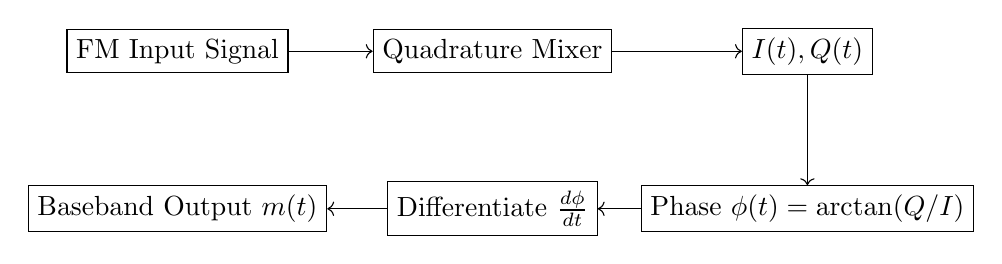
\begin{tikzpicture}[node distance=2cm,auto]
    % Nodes
    \node (in) [draw, rectangle] {FM Input Signal};
    \node (mix) [draw, rectangle, right of=in, node distance=4cm] {Quadrature Mixer};
    \node (iq) [draw, rectangle, right of=mix, node distance=4cm] {$I(t), Q(t)$};
    \node (phase) [draw, rectangle, below of=iq, node distance=2cm] {Phase $\phi(t) = \arctan(Q/I)$};
    \node (diff) [draw, rectangle, left of=phase, node distance=4cm] {Differentiate $\frac{d\phi}{dt}$};
    \node (out) [draw, rectangle, left of=diff, node distance=4cm] {Baseband Output $m(t)$};

    % Connections
    \draw[->] (in) -- (mix);
    \draw[->] (mix) -- (iq);
    \draw[->] (iq) -- (phase);
    \draw[->] (phase) -- (diff);
    \draw[->] (diff) -- (out);
\end{tikzpicture}
\end{center}

\section*{Relay Feedback 自動整定(Åström--Hägglund)}

\subsection*{關鍵公式}
理想繼電器輸出幅度為 $\pm h$,若閉迴路產生穩定極限循環,輸出正弦近似幅度為 $a$、週期為 $P_u=2\pi/\omega_u$,則
\[
N(a)=\frac{4h}{\pi a},\qquad
G(j\omega_u)\,N(a)=-1
\]
由此可得臨界增益
\[
K_u=\frac{4h}{\pi a}.
\]

\subsection*{控制框圖}
\begin{center}
\begin{tikzpicture}[
  block/.style={draw,rectangle,minimum height=10mm,minimum width=18mm,align=center},
  sumsym/.style={draw,circle,inner sep=0pt,minimum size=6mm}, % 這行是定義 sumsmy 樣式
  >={Stealth}
]
% Nodes
\node[block] (ref) {參考 $r(t)$};
\node[sumsym, right=12mm of ref] (adder) {$\sum$};
\node[block, right=12mm of adder] (relay) {繼電器\\$\pm h$};
\node[block, right=12mm of relay] (plant) {被控對象\\$G(s)$};
\node[block, right=12mm of plant] (meas) {輸出 $y(t)$};

% Connections
\draw[->] (ref) -- (adder);
\draw[->] (adder) -- node[above] {$e(t)$} (relay);
\draw[->] (relay) -- node[above] {$u(t)$} (plant);
\draw[->] (plant) -- (meas);
\draw[->] (meas.south) |- ++(0,-12mm) -| node[pos=0.75,below] {$-$} (adder.south);

\end{tikzpicture}
\end{center}

\subsection*{說明}
\begin{itemize}
  \item 將原控制器暫時以繼電器取代,閉迴路自然激發極限循環。
  \item 量測輸出振幅 $a$ 與週期 $P_u$,由 $K_u=\tfrac{4h}{\pi a}$ 推得臨界增益,再套用 Ziegler--Nichols 或其他整定規則得到 PID 參數。
\end{itemize}
================================================================
這個FM解調器使用$\pi$/4延遲的原理如下:

\section{FM信號的特性}

FM信號可以表示為:
\begin{equation}
s(t) = A \cos(\omega_c \cdot t + \phi(t))
\end{equation}
其中$\phi(t)$包含調變信息。

\section{$\pi$/4延遲的作用}

\subsection{相位差分析}
當信號經過$\pi$/4延遲後:
\begin{itemize}
    \item 原信號:$s(t) = A \cos(\omega_c \cdot t + \phi(t))$
    \item 延遲信號:$s\left(t - \frac{\pi}{4\omega_c}\right) = A \cos\left(\omega_c \cdot t - \frac{\pi}{4} + \phi\left(t - \frac{\pi}{4\omega_c}\right)\right)$
\end{itemize}

\subsection{乘法器的輸出}
兩信號相乘後:
\begin{align}
s(t) \times s\left(t - \frac{\pi}{4\omega_c}\right) &= \frac{A^2}{2} \times \left[\cos\left(2\omega_c \cdot t - \frac{\pi}{4} + \phi(t) + \phi\left(t - \frac{\pi}{4\omega_c}\right)\right)\right. \nonumber \\
&\quad \left.+ \cos\left(\frac{\pi}{4} - \phi(t) + \phi\left(t - \frac{\pi}{4\omega_c}\right)\right)\right]
\end{align}

\subsection{低通濾波後}
高頻項被濾除,剩下:
\begin{equation}
\text{Output} \propto \cos\left(\frac{\pi}{4} - \left[\phi(t) - \phi\left(t - \frac{\pi}{4\omega_c}\right)\right]\right)
\end{equation}

\section{為什麼選擇$\pi$/4?\{should be modiffied to T/4\}}

\subsection{最佳靈敏度}
\begin{itemize}
    \item 在$\pi$/4相位差處,cos函數的斜率最大
    \item 提供最佳的相位變化到電壓變化的轉換靈敏度
    \item 線性度在小信號範圍內最好
\end{itemize}

\subsection{數學最佳化}
對於小的相位變化$\Delta\phi$:
\begin{equation}
\cos\left(\frac{\pi}{4} - \Delta\phi\right) \approx \cos\left(\frac{\pi}{4}\right) + \sin\left(\frac{\pi}{4}\right) \cdot \Delta\phi = \frac{\sqrt{2}}{2} + \frac{\sqrt{2}}{2} \cdot \Delta\phi
\end{equation}

$\pi$/4時,$\sin\left(\frac{\pi}{4}\right) = \frac{\sqrt{2}}{2}$為最大值。

\subsection{頻率檢測}
瞬時頻率偏差:
\begin{equation}
\Delta\omega = \frac{d\phi}{dt} \approx \frac{\phi(t) - \phi(t - T)}{T}
\end{equation}
其中$T = \frac{\pi}{4\omega_c}$

\section{電路優勢}

\subsection{簡單實現}
\begin{itemize}
    \item 只需要一個延遲線
    \item 一個乘法器
    \item 一個低通濾波器
\end{itemize}

\subsection{寬頻帶響應}
\begin{itemize}
    \item 適用於各種調變指數
    \item 頻率響應相對平坦
\end{itemize}

\subsection{線性度好}
\begin{itemize}
    \item 在工作範圍內接近線性
    \item 失真較小
\end{itemize}

\section{實際考量}

\subsection{延遲精度}
$\pi$/4延遲必須精確,通常使用:
\begin{itemize}
    \item 傳輸線
    \item LC延遲線
    \item 數位延遲
\end{itemize}

\subsection{頻寬限制}
延遲時間限制了可解調的最高頻率。

\subsection{溫度穩定性}
延遲線的溫度係數會影響性能。

\section{性能比較}

\begin{center}
\begin{tabular}{>{\centering\arraybackslash}m{3cm} >{\raggedright\arraybackslash}m{8cm}}
\toprule
\textbf{延遲角度} & \textbf{特性} \\
\midrule
0$^{\circ}$ & 無解調輸出 \\
$\pi$/6 & 靈敏度較低 \\
$\pi$/4 & \textbf{最佳靈敏度和線性度} \\
$\pi$/3 & 靈敏度下降 \\
$\pi$/2 & 零輸出點 \\
\bottomrule
\end{tabular}
\end{center}

\section{總結}

$\pi$/4延遲是FM解調器中的最佳選擇,因為它:
\begin{enumerate}
    \item 提供最大的檢測靈敏度
    \item 確保良好的線性度
    \item 實現簡單且可靠
    \item 在數學上為最佳工作點
\end{enumerate}

這就是為什麼商用FM解調器普遍採用$\pi$/4延遲線設計的原因。


\end{document}